
\chapter{The Campaign}

\subsection{Tempestas}

At the start of the campaign, the DM needs to decide on a reason for the characters to be coming into Tempestas. This can be any good reason that fits with the player backstories or one from the following list. Tempestas is a large city with many things to do. The city will start closed off due to the impending threat of the Celestials attacking nearby cities. From Tempestas, the players can be lead to Aurushire. Different reasons can lead them to Aurushire such as the sport of the jungles or the search for the Trinity stones. Little do they know that the Trinity stones are the key to obtaining the San'graal to defeat the Celestials.

The players can start out in Tempestas either by living there, being in the prison there, or arriving there by spice trade (depending on the character backgrounds). While in Tempestas, they can encounter a few important characters such as Dastan and the fortuneteller. While in Tempestas, a Prior of the Celestas will also arrive and start his preaching. 

\subsection{Journey to Aurushire}

\begin{commentbox}{Journey to Aurushire}
	\begin{description}
		\item[For the Stones] Legend has it that there are rare and priceless artifacts hidden on Statu. It is possible that the player could be hunting the legends which have lead them to Aurushire.
		\item[The Rare Sport of Rem Silva] It is possible that the rare game in Rem Silva was spoken of and the players could be after the rare sport that resides in this area.
	\end{description}
\end{commentbox}

After leaving Tempestas by boat (If the party gets to this), they will have some rest time on the ship they are on. The tripe is generally only about a day or two away from Statu, however the party will encounter rough weather. The rough weather will turn into a massive storm in which the ship will be knocked around, back and forth. The party will be knocked unconscious and awake on the coast due east on Aurushire (without knowing of course) with only the players that are in their party and none of the NPCs from the ship. The cost will have rock and cliff faces to their east, and rough forest and mountains (appears unclimbable) to the North. Their only option is the the west. The west will lead into the Convallis swamp and marsh area's which is directly east of the Naga encampments. A thick fog will appear as they are traveling and they will need to navigate through rough swampy regions where they will encounter serpent Naga forces and some magical beasts like a witch hunter. After navigating through this region, the party will arrive and Aurushire, battered and beaten.

After arriving at Aurushire, there are many options for the players. There is an Inn (Prancing Pony Inn), where they can get rest. There are farms, where the players could potentially work. There are the mines, run by a Pandaren brother, where players could also work. There is a blacksmith, which is run by one of the three Pandaren brothers. There is the brewery/tavern, which is run by another Pandaren brother for players to socialize, learn, and relax. There is also Bob's Guns. Bob is a strange fella who claims is he from a more modern time. He has things that you cannot find anywhere else. To the northeast there is an old witch named Yaga. To the northwest a wizard named Baba. Together the two are sometimes referred to as the Ying-Yang. For one appears good, and one appears the opposite. Though this name comes from the matter of looks, and not actions. 

\subsection{Baba}

Baba is a powerful wizard who has spent many lifetimes studying the flow of time and impacts of the time stone on the surrounding regions. Baba can be found throughout the time line as different versions of herself. At one point she found a way to manipulate the temporal and spacial fluctuations throughout the region to create copies of herself in different space-times. From this, there are Baba's hidden throughout the time line all living as separate entities. 

Baba's role can be whatever the DM likes. She was intended to persuade the users to seek the trinity stones. Along with this, Baba knows the powers and trickery of the stones and would not believe the party is ready no matter how experienced. Because of this, she can teleport them to various locations for trials such as the halls of no end \ref{maps} or the various surrounding regions. 

\begin{center}
	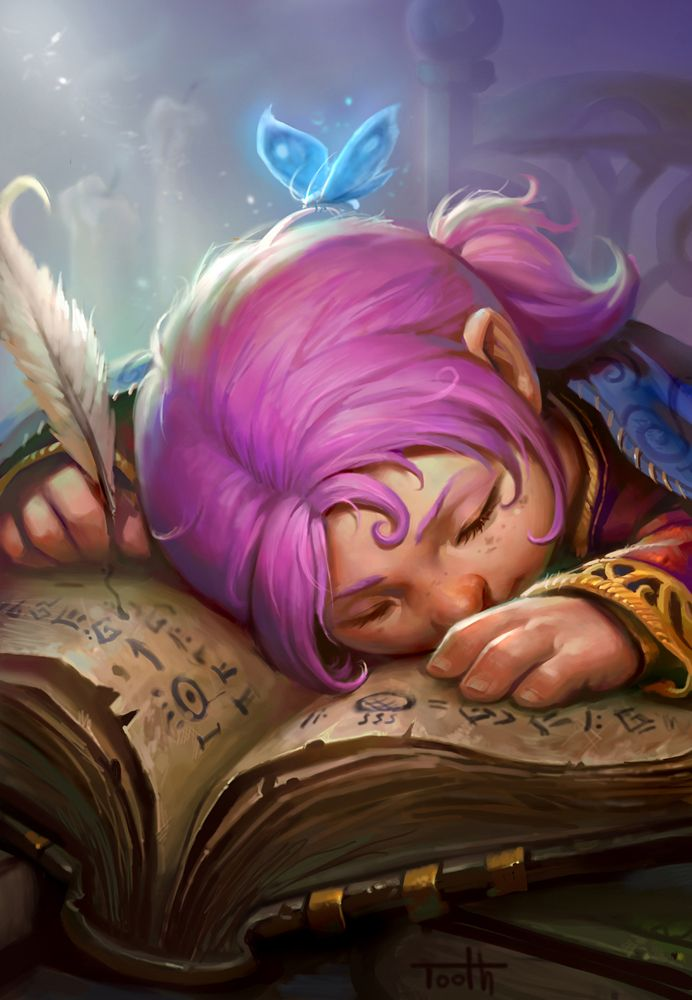
\includegraphics[width=0.5\linewidth]{img/baba.jpg}
\end{center}

\begin{monsterbox}{Baba}
	\begin{hangingpar}
		\textit{Gnome Wizard, Neutral Good}
	\end{hangingpar}
	\dndline%
	\basics[%
	armorclass = 24,
	hitpoints  = 302,
	speed      = 60 ft
	]
	\dndline%
	\stats[
	STR = \stat{8}, % This stat command will autocomplete the modifier for you
	DEX = \stat{16},
	CON = \stat{19},
	INT = \stat{20},
	WIS = \stat{20},
	CHA = \stat{19}
	]
	\dndline%
	\details[%
	% If you want to use commas in these sections, enclose the
	% description in braces.
	% I'm so sorry.
	languages = {Common, Elvish, Dwarvish, Gnomish, Halfling, Orc, Pandaren, Celestial, Draconic, Primordial},
	challenge = 20
	]
	\dndline%
	\begin{monsteraction}[Telekinesis]
		The ability to move objects with your mind. There is no limitation to how the objects can be moved if the objects belong to you.
	\end{monsteraction}	
	\begin{monsteraction}[Cerebral Warp]
		You can place humanoids into a deep illusion that seems completely real. The subjects cannot be harmed in the illusion.
	\end{monsteraction}	
	\begin{monsteraction}[Illusionary Presence]
		When you are near others, you feel to them to be in multiple places at once. If struck by a melee attack, you can relocate to an alternate location within 10 feet.
	\end{monsteraction}
	\begin{monsteraction}[Precision Striking]
		When you attack, you can choose hwo much damage to deal up to the amount shown on the attack roll.
	\end{monsteraction}
	\monstersection{Actions}
	\begin{monsteraction}[Spells]
		A lot of spells.
	\end{monsteraction}
	\begin{monsteraction}[Temporal Shift]
		Baba can send herself and another creature into the past for 3 minutes and 14 seconds. 
	\end{monsteraction}
	\monstersection{Description/Information}
	Baba lives in seclusion. She is an extremely small gnome that does not mind helping others when asked. She is extremely intelligent and powerful, even though she does not look it. Baba is very old, however, very well kept and appears young.
\end{monsterbox}

\begin{commentbox}{Baba's Wizard Hat}
	Baba's hat has a mind of it's own. As a good way to show the personality of Baba, the Hat she wears can move on it's own, showing emotion and performing magical acts. As an example, if someone says something surprising to Baba, the hat itself can do a sort of 'eyebrow raise'. Also, when Baba walks forward, the hat could remain stationary and come off of her head if it's surprised or distracted. The hat is similar to the hat from Harry Potter only it cannot speak and does not have a mouth or eyes.
\end{commentbox}

\begin{commentbox}{Baba as Morgana}
	Within the campaign, Baba can be used as Morgana. Myrddin was much more crafty, intelligent, and clever than Morgana was. In regards to creating the San'graal, he created the Trinity stones and was able to manipulate and parse through temporal (time) events. Due to this, he was able to hide his clues throughout time. 
	
	Morgana realized this but did not have the same understanding and Myrddin. She found a way to manipulate the trinity stones in order to essentially clone herself throughout different space-times. This has allowed Baba to wait in different temporal locations for mysteries of Myrddin.
\end{commentbox}

\begin{commentbox}{Baba as Morgana's sister}
	Within the campaign, Baba can be used as Morgana's sister. Myrddin was much more crafty, intelligent, and clever than Morgana was. In regards to creating the San'graal, he created the Trinity stones and was able to manipulate and parse through temporal (time) events. Due to this, he was able to hide his clues throughout time. 
	
	Morgana realized this but did not have the same understanding and Myrddin. Her sister, Baba found a way to manipulate the trinity stones in order to essentially clone herself throughout different space-times. This has allowed Baba to wait in different temporal locations for mysteries of Myrddin. After thinking her sister was a bit crazy for all of the things she spouted off about Myrddin, later in her life she discovered anomalies that supported the things her sister claimed. She eventually turned towards studying the mysteries left by Myrddin.
\end{commentbox}

\begin{commentbox}{Baba's Tower}
	Baba resides in a mage tower that lies about a day's journey to the northwest of Aurushire. The tower is multileveled and has a winding wooden staircase that leads all the way to the top level of the tower. The tower contains many different books and brewing stations among it's level. The tower has a hollow center where the top can be seen from the bottom. The top level is larger than all of the other but other than that level, the tower slightly narrows from bottom to top. At the top level, Baba has a view of a large portion of the surrounding regions ans it reaches just above the tree line. One thing the party may try to do is look for books throughout the place. Baba has lifetimes she has been studying and can speak many languages. Because of this, she has books of all sorts of languages. On the first level of the tower is living area's, with couches, a fireplace, tables, chairs and a very cozy and comfortable looking arrangement. As the levels go up, there are different forms of information leading to the top level where Baba has all of the high level information that she needs quick access to for studying.
\end{commentbox}

\begin{commentbox}{Kharazan}
	Kharazan is a tower that is about a 3 days journey to the northeast of Aurushire. Kharazan is a huge but semi-deserted castle. The place is old and many parts of it are broken down. There are many rooms in it such as a ballroom, full storehouse, large dining halls, dungeons, libraries, theaters, etc (Modeled similarly to the Kharazan castle in World of Warcraft). This place is where Yaga resides deep into one of the libraries of the castle up in one of the highest castles. Most of the things found within the castle are dust covered and appear to have not been used in many years.
	
	At the entrance of the castle lies a sleeping curator. This is a robotic like creature (very large) that will awaken if anyone enters the place. This curator is not hostile unless provoked or protecting the castle. This curator serves the master of the castle and can be used to give information or lead the party to where they need to go. Throughout the castle, there is a faint tune playing continually that is caused by an enchantress' spell created after the castle was abandoned.
\end{commentbox}

\begin{center}
	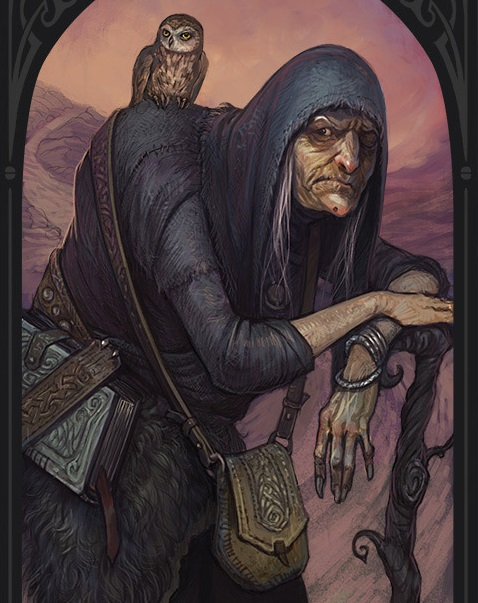
\includegraphics[width=0.5\linewidth]{img/Yaga.jpg}
\end{center}

\begin{monsterbox}{Yaga}
	\begin{hangingpar}
		\textit{?? ??, Neutral ??}
	\end{hangingpar}
	\dndline%
	\basics[%
	armorclass = ??,
	hitpoints  = ??,
	speed      = ?? ft
	]
	\dndline%
	\stats[
	STR = \stat{}, % This stat command will autocomplete the modifier for you
	DEX = \stat{},
	CON = \stat{},
	INT = \stat{},
	WIS = \stat{},
	CHA = \stat{}
	]
	\dndline%
	\details[%
	% If you want to use commas in these sections, enclose the
	% description in braces.
	% I'm so sorry.
	languages = {Common},
	challenge = 20
	]
	\dndline%
	\monstersection{Description/Information}
	Yaga is an old sorcerer. Not much is known about her. She is tall and frail (or at least appears so). It is impossible to tell anything about her from looking at her. This NPC is a wild card. It can be used with the story as seen fit (save the important things she contains to the campaign).
\end{monsterbox}

\begin{commentbox}{The Ying-Yang}
	The Ying-Yang (Baba and Yaga) plays an important part of this campaign. 
	
	Baba is a wizard that is interested in helping the party learn. She contains a vast library of knowledge and knows much about the Trinity stone legends and myths. She can assist the party in learning more. Similarly, she will insist the party is not ready if they claim they are seeking Athereu and if they insist they are will put the party through tests to confirm it. One test is to teleport the party to the halls of no end. Another would be to send them into Rem Silva after something that would help them on their journey. These challenges would be designed to assist them in their journey. 
	
	Yaga is an old witch. She appears to contain vast knowledge of the trinity stone legends as well, but acts as if she knows nothing. She can assist the party in acquiring clues and items that will help find their way to their goal. Specifically, she contains a map of Aethereu (the inside) which appears as a blank piece of paper until entering Aethereu. This map is pivotal to easily navigating the chamber. Alternatively, she can contain clues regarding successful passage through The Pluvian Forest, along with Baba.
\end{commentbox}



\begin{commentbox}{Samilah}
	Samilah, which is a name derived from Samson and Delilah meaning ``shining night''. She can be placed into the campaign in many ways but serves as the mortal embodiment of the Celestials. Her main goal is to destroy the San'graal which is the only mortal weapon known to be able to destroy the Celestials. She can disguise herself as any other sentient being and has a necklace that will protect her from any harm. She is mentally disciplined so that her mind cannot be messed with and has nearly unlimited capabilities. After destroying the San'graal she will lead the Celestial army in the conquest of Orilla.
	\begin{center}
		
\includegraphics[width=0.7\linewidth]{img/samilah.jpg}
	\end{center}
\end{commentbox}

\begin{commentbox}{Eternal Neokoros}	
	The Eternal Neokoros is a creature modeled after the Eternal Neokoros from the Halo series. It's appearance and voice mirror that of the Halo creature but it's purpose is expanded for use in this campaign. This creature has existed since before humanity. It lives deep in the Earth and prefers warm and humid climates. The creature is not very mobile as far as relocating its self, however it is extremely agile in battles as it has a large amount of tendrils that can poison, paralyze, attack and more to anything it desires. The creature typically travels through a cave system that exists on volcanic fault lines under oceans. 
	
	Where the creature can appear in the campaign can vary but is typically if a player, or the party finds themselves adrift in the ocean or body of water. The creature needs a large amount of time to surface and show itself. It can also extend its tendrils vast distances and could collect objects or people from long distances away (such as under a body of water). It does need a large amount of time to do this so the target would need to be immobilized or inanimate. The Eternal Neokoros is well aware of most things occurring on the surface of the planet as it can hear through rock and metal and continually watches and learns as the species of the planet develop. The Eternal Neokoros has rarely been seen throughout history but some Legends and stories have arose from it such as that of the Loch'Ness Monster and that of a flood invasion.
	
	\begin{center}
		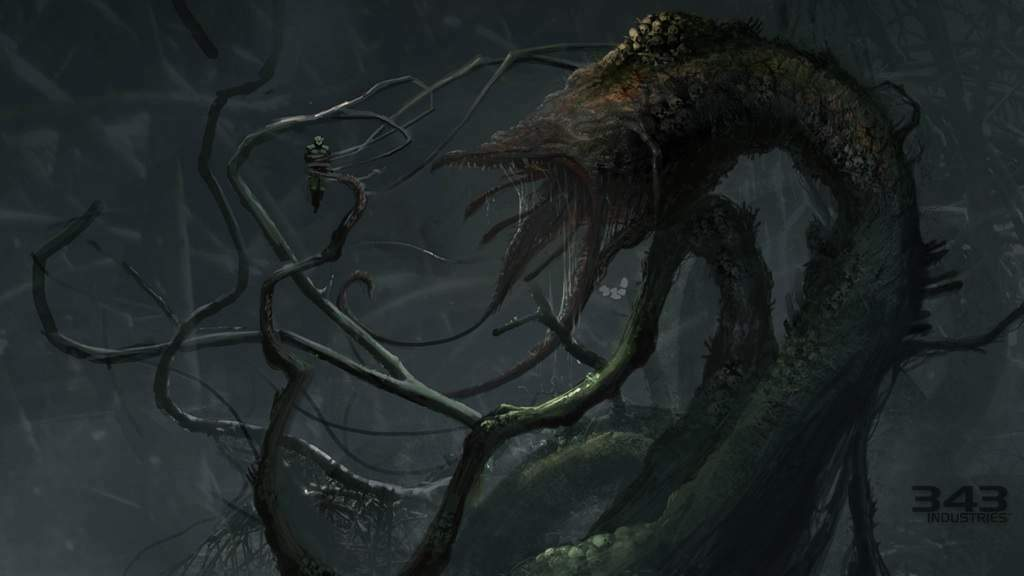
\includegraphics[width=0.6\linewidth]{img/gravemind.jpg}
	\end{center}

	The Eternal Neokoros can create an offspring Neokoros within a host creature. The offspring has a faint link to the Eternal Neokoros and shares an eternal bond that links the creatures through space. If the offspring of the Eternal Neokoros is killed by a sentient being, the Eternal Neokoros will feel the pain of losing its child and seek revenge.
\end{commentbox}

\begin{monsterbox}{Eternal Neokoros}
	\begin{hangingpar}
		\textit{Huge Huge Monstrosity, Chaotic Neutral}
	\end{hangingpar}
	\dndline%
	\basics[%
	armorclass = 22 (Body) + 25 (tendrils),
	hitpoints  = 460,
	speed      = 5 ft (self) + 50 ft (tendrils)
	]
	\dndline%
	\stats[
	STR = \stat{21}, % This stat command will autocomplete the modifier for you
	DEX = \stat{18},
	CON = \stat{30},
	INT = \stat{30},
	WIS = \stat{24},
	CHA = \stat{16}
	]
	\dndline%
	\begin{monsteraction}[Eternal Wisdom]
		The eternal nature of this beast gives it infinite capabilities with mental challenges. The creature cannot fail wisdom checks/saves.
	\end{monsteraction}	
	\begin{monsteraction}[Legendary Action]
		If the eternal creature fails a saving throw, it can instead choose to succeed. This can occur up to 2 times a day.
	\end{monsteraction}
	\begin{monsteraction}[Unpredictable Tendril Presence]
		Because of the number of tendrils and size of the creature, it gets four separate turns in the initiative order. One for the Eternal Neokoros and three for each major tendril. 
	\end{monsteraction}	
	\begin{monsteraction}[Eternal Horror]
		The creature appears extremely horrifying and terrifying. Any creature seeing it must make a DC18 constitution save. If the target fails it is frightened and cannot take actions until an action is taken against them. 
	\end{monsteraction}	
	
	\monstersection{Actions}
	\begin{monsteraction}[Eternal Attack Pattern]
		The creature is so intelligent that it can manipulate all of it's tendrils in a precise manner and coordinate attacks flawlessly. Because of this it can take 3 attacks or actions per turn.
	\end{monsteraction}
	\begin{monsteraction}[Eternal Whip]
		The creature can whip a tendril towards a target. +8 hit and deals 4d6 damage. This will also paralyze any target that is grappled.
	\end{monsteraction}
	\begin{monsteraction}[Eternal Bind]
		\begin{itemize}
			\item The creature can burrow one of it's tendrils through the ground and wrap itself around a player without them realizing. The tendril can then pull the target's leg into the ground (except through rock or metal) causing the target to be grappled by the ground.
			\item Alternatively, the creature can grapple a being with one of its tendrils.
		\end{itemize}
	\end{monsteraction}
	\begin{monsteraction}[Paralytic Substance]
		The creature can excrete a goo-like compound from any of it's tendrils that can paralyze an opponent. 
	\end{monsteraction}
	\begin{monsteraction}[Throw Creature]
		If a target is grappled by one of the creatures tendrils, it can throw the target causing 3d10+4 damage.
	\end{monsteraction}
	\begin{monsteraction}[Eternal Deafening]
		The creature can use an action to impose a psychic attack on every foe it's facing simultaneously. All creatures must make a DC 18 Wisdom save. On a succeed, they obtain a headache and a nose bleed and take 2 damage. On a fail, they also take 1d8 damage.
	\end{monsteraction}
	
	\details[%
	% If you want to use commas in these sections, enclose the
	% description in braces.
	% I'm so sorry.
	languages = {All},
	challenge = 20
	]
	\dndline%
	\monstersection{Description/Information}
	The Eternal Neokoros can only be seen by killing the Neokoros offspring, thus provoking revenge. This creature is extremely large and essentially requires an army to defeat.	
		
	\begin{center}
		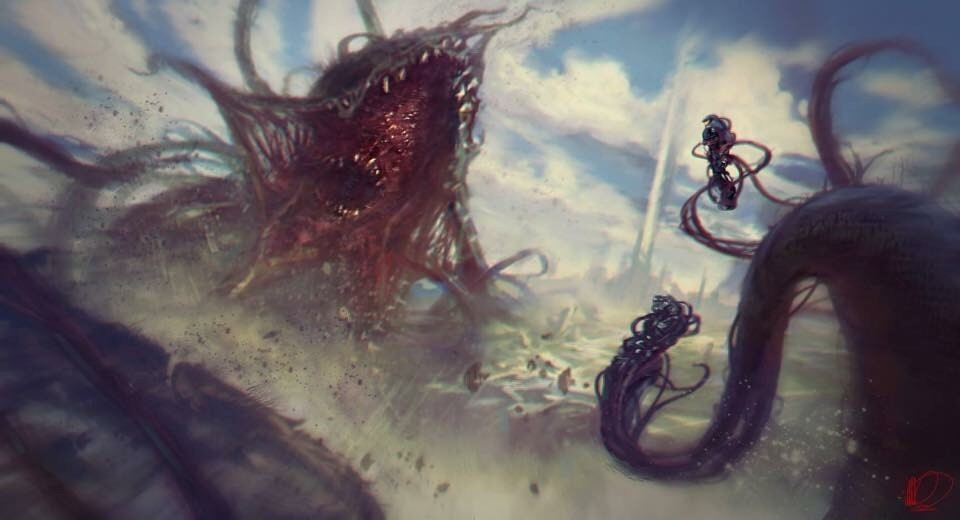
\includegraphics[width=0.475\linewidth]{img/gravemind-battle.jpg} 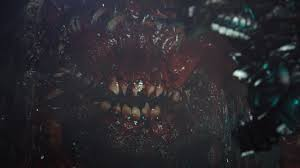
\includegraphics[width=0.46\linewidth]{img/gravemind-face.jpg}
	\end{center}
\end{monsterbox}

\begin{monsterbox}{Neokoros Tendril}
	\begin{hangingpar}
		\textit{Huge Huge Monstrosity, Chaotic Neutral}
	\end{hangingpar}
	\dndline%
	\basics[%
	armorclass = 21 (Body) + 23 (tendrils),
	hitpoints  = 180,
	speed      = 5 ft (self) + 40 ft (tendrils)
	]
	\dndline%
	\stats[
	STR = \stat{21}, % This stat command will autocomplete the modifier for you
	DEX = \stat{18},
	CON = \stat{30},
	INT = \stat{30},
	WIS = \stat{24},
	CHA = \stat{16}
	]
	\dndline%
	\begin{monsteraction}[Eternal Connection]
		The Tendril has all of the same abilities as the Eternal Neokoros as it is attached to it.
	\end{monsteraction}	
	
	\monstersection{Actions}
	\begin{monsteraction}[Eternal Devour]
		If a creature is close to the tendril, it can open up with multiple layers of teeth and attempt to devour a creature. The creature must make a DC16 dexterity saving throw or take 3d6+4 damage. If this kills the target, they are devoured and instantly gain three failed death saves.
	\end{monsteraction}
	\begin{monsteraction}[Eternal Whip]
		The creature can whip a tendril towards a target. +8 hit and deals 4d6 damage. This will also paralyze any target that is grappled.
	\end{monsteraction}
	\begin{monsteraction}[Eternal Bind]
		\begin{itemize}
			\item The creature can burrow one of it's tendrils through the ground and wrap itself around a player without them realizing. The tendril can then pull the target's leg into the ground (except through rock or metal) causing the target to be grappled by the ground.
			\item Alternatively, the creature can grapple a being with one of its tendrils.
		\end{itemize}
	\end{monsteraction}
	\begin{monsteraction}[Paralytic Substance]
		The creature can excrete a goo-like compound from any of it's tendrils that can paralyze an opponent. 
	\end{monsteraction}
	\begin{monsteraction}[Throw Creature]
		If a target is grappled by one of the creatures tendrils, it can throw the target causing 3d10+4 damage.
	\end{monsteraction}
	\begin{monsteraction}[Eternal Deafening]
		The creature can use an action to impose a psychic attack on every foe it's facing simultaneously. All creatures must make a DC 18 Wisdom save. On a succeed, they obtain a headache and a nose bleed and take 2 damage. On a fail, they also take 1d8 damage.
	\end{monsteraction}
	
	\details[%
	% If you want to use commas in these sections, enclose the
	% description in braces.
	% I'm so sorry.
	languages = {All},
	challenge = 15
	]
	\dndline%
	\monstersection{Description/Information}
	The Eternal Neokoros Tendril appears when the Eternal Neokoros is around. This is a major Tendril connected to the Eternal Neokoros which has it's own set of tendrils that send out attacks.
\end{monsterbox}

\begin{commentbox}{Neokoros}
	The Eternal Neokoros can lay an offspring by intertwining a bit of its DNA into another creatures nervous system. The offspring is known as Neokoros and grows in strength as the player grows. This offspring can act on it's own and becomes part of its host (similar to Venom from the spider-man series). As time passes, it can develop a relationship with the host or overtake them. Instead of having it's own turn order and stats, it instead increases the stats of a player when active. The creature can activate when it desires. If the player has a relationship with the creature, it can have some influence on when the creatures abilities activate. The main purpose of the creature is to do whatever the Eternal Neokoros gave it as its mission. For the purposes of this campaign, it's mission is to find the Trinity Stones and destroy the Celestials, though it doesn't know this precisely until the creature grows and develops more. The consciousness of the creature will slowly unravel over time.
	
	The appearance of the Neokoros can vary greatly. One method of such appearance is to appear as an alien eye within the host. The eye would have small purple veins that were not there before the infection that stem from the eye on the side of the hosts head. The parasite cannot be removed without killing the host player. Abilities of the Neokoros are determined by the level of the host creature.
	
	The Neokoros can heal the player for 1d6 per host level at any point it chooses. This can occur once per long rest.
	
	\begin{description}
		\item[Level 1:] The creature can telepathically communicate with the player, occasionally speaking single words or phrases.
		\item[Level 2:] The creature can sometimes move the host when the host is unconscious.
		\item[Level 3:] The creature can sometimes provide a strength success when the host is acting with their reflexes. 
		\item[Level 4:] The creature can sometimes provide an increase in combat abilities of the player.
		\item[Level 5:] The creature begins to communicate more with the host alerting the host that it has a conscious.
		\item[Level 5:] The creature can sometimes control the player while the player is conscious.
		\item[Level 6:] The creature can create visual hallucinations for the player.
		\item[Level 7:] The creature will try to either manipulate or befriend the host.
		\item[Level 8:] The creature provides a permanent +1 to strength to the host as it begins to alter the host internal cellular structure.
		\item[Level 9:] 
 	\end{description}
\end{commentbox}
